\documentclass[main.tex]{subfiles} % Subfile-Class



% ============================================================================== %
%                            Subfile document                                    %
% ============================================================================== %

\begin{document}

% Template

\subsubsection{Liniensensor}

Im folgenden Abschnitt wird die Entwicklung und Evaluierung eines Liniensensors
dokumentiert. Ziel ist es, einen einfach auszuwertenden Sensor zu entwickeln,
der das vorgegebene Klebeband (\textit{Tesa Gewebeband 4651}) problemlos von
der Wettkampfbahn unterscheiden kann.

Ein eigener Liniensensor wird entwickelt, da das Verlassen der Strecke als
hohes Risiko empfunden wird. Die Eigenentwicklung eines Liniensensors
ermöglicht daher eine hohe Flexibilität. Denn für ein massgeschneidertes
Produkt können alle Komponenten selbst ausgewählt werden können.

% ===================================================================================
\subsubsection*{Anforderungen}

Das Klebeband soll auf einem rötlich gefliesten Untergrund detektiert werden.
Eine besondere Herausforderung stellen die gleichfarbigen Längs- und Querfugen
der Fliesen dar. Dieser Untergrund ist in der Abbildung
dargestellt~\ref{fig:Untergrund_Wettkampf}.

\begin{figure}[H]
    \centering
    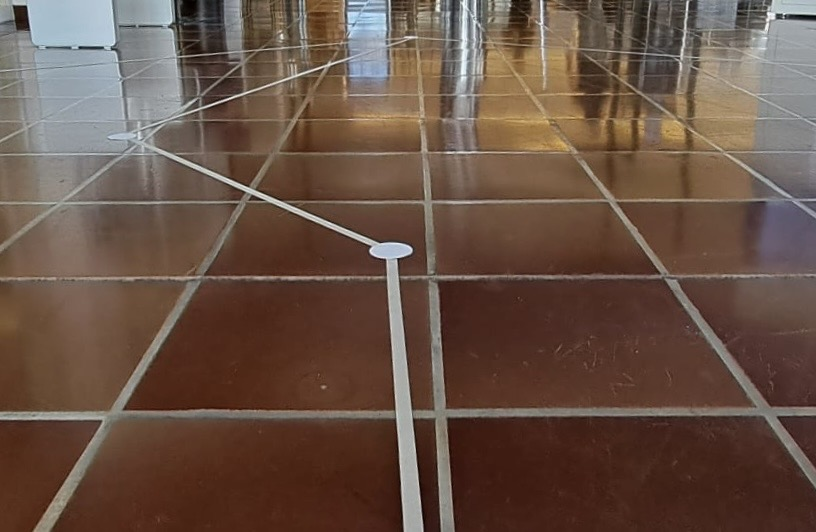
\includegraphics[width=0.75\textwidth]{fig_Strecke_Tracken/Bild_Untergrund.jpg}
    \caption{Untergrund während des Wettkampfs}~\label{fig:Untergrund_Wettkampf}
\end{figure}

% ===================================================================================

\subsubsection*{Aufbau und Auswertung}
Der Liniensensor besteht aus acht einzelnen Messzellen. Die Anzahl der Messzellen wurde so
gewählt, dass ein möglichst grosser Bereich vom Sensor abgedeckt wird, aber nicht zu viele
Pins für die Auswertung benötigt werden. Es sollten immer genau zwei Messzellen direkt über
dem Klebeband ausgerichtet sein. Jede einzelne Messzelle besitzt eine Leuchtdiode und einen
zugehörigen Fototransistor. Je mehr Licht auf den Fototransistor fällt, desto höher ist der
Strom, der durch ihn fliesst. Da der Fototransistor als Konstantstromquelle interpretiert
werden kann, wird der Spannungspegel zwischen Widerstand und Transistor ausgewertet.

Ein hoher Strom durch den Fototransistor führt dazu, dass der Transistor
versucht, mehr Strom zu liefern, als ihm der Widerstand 'erlaubt'. Er gerät
dadurch in Sättigung und das Potential wird sehr stark gegen GND gezogen. Ist
die Reflexion und damit der Strom dagegen gering, lässt der Fototransistor
weniger Strom durch, als der Widerstand eigentlich erlauben würde, und der
Spannungspegel bewegt sich stark in Richtung 3,3V. Diese Spannungen werden dann
mit Hilfe von Analog-Digital-Wandlern (ADCs) ausgewertet. In
Abbildung~\ref{fig:Auswertung_Liniensensor1} ist die Auswertung schematisch
dargestellt.
\begin{figure}[H]
    \centering
    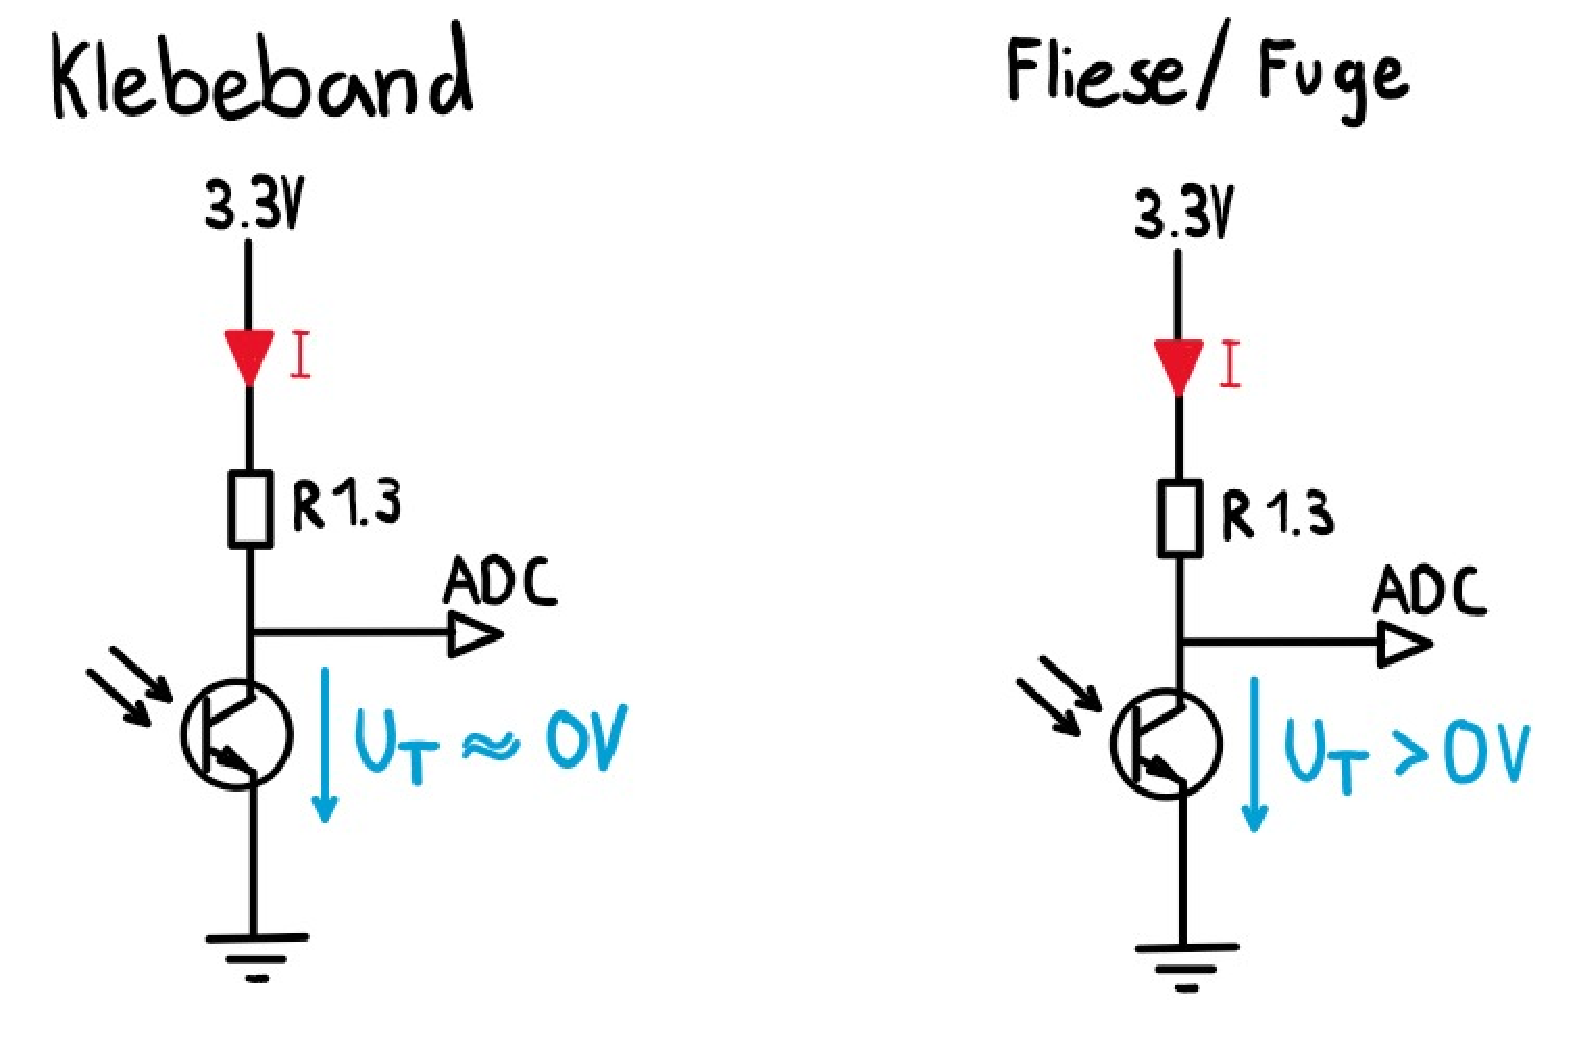
\includegraphics[width=0.5\textwidth]{fig_Strecke_Tracken/Auswertung_Liniensensor.pdf}
    \caption{Konzept der Auswertung mittels ADC}~\label{fig:Auswertung_Liniensensor1}
\end{figure}

% ===================================================================================

\subsubsection{Liniensensor als PCB}

Damit der Liniensensor möglichst praxisnah getestet werden kann, wird dieser
als PCB mit KiCad erstellt. Dabei werden die oben formulierten Anforderungen
und Dimensionierungen eingehalten. In Abbildung~\ref{fig:Liniensensor_Top} ist
die Draufsicht und in Abbildung~\ref{fig:Liniensensor_Bottom} die Untersicht
dargestellt.

\begin{figure}[H]
    \centering
    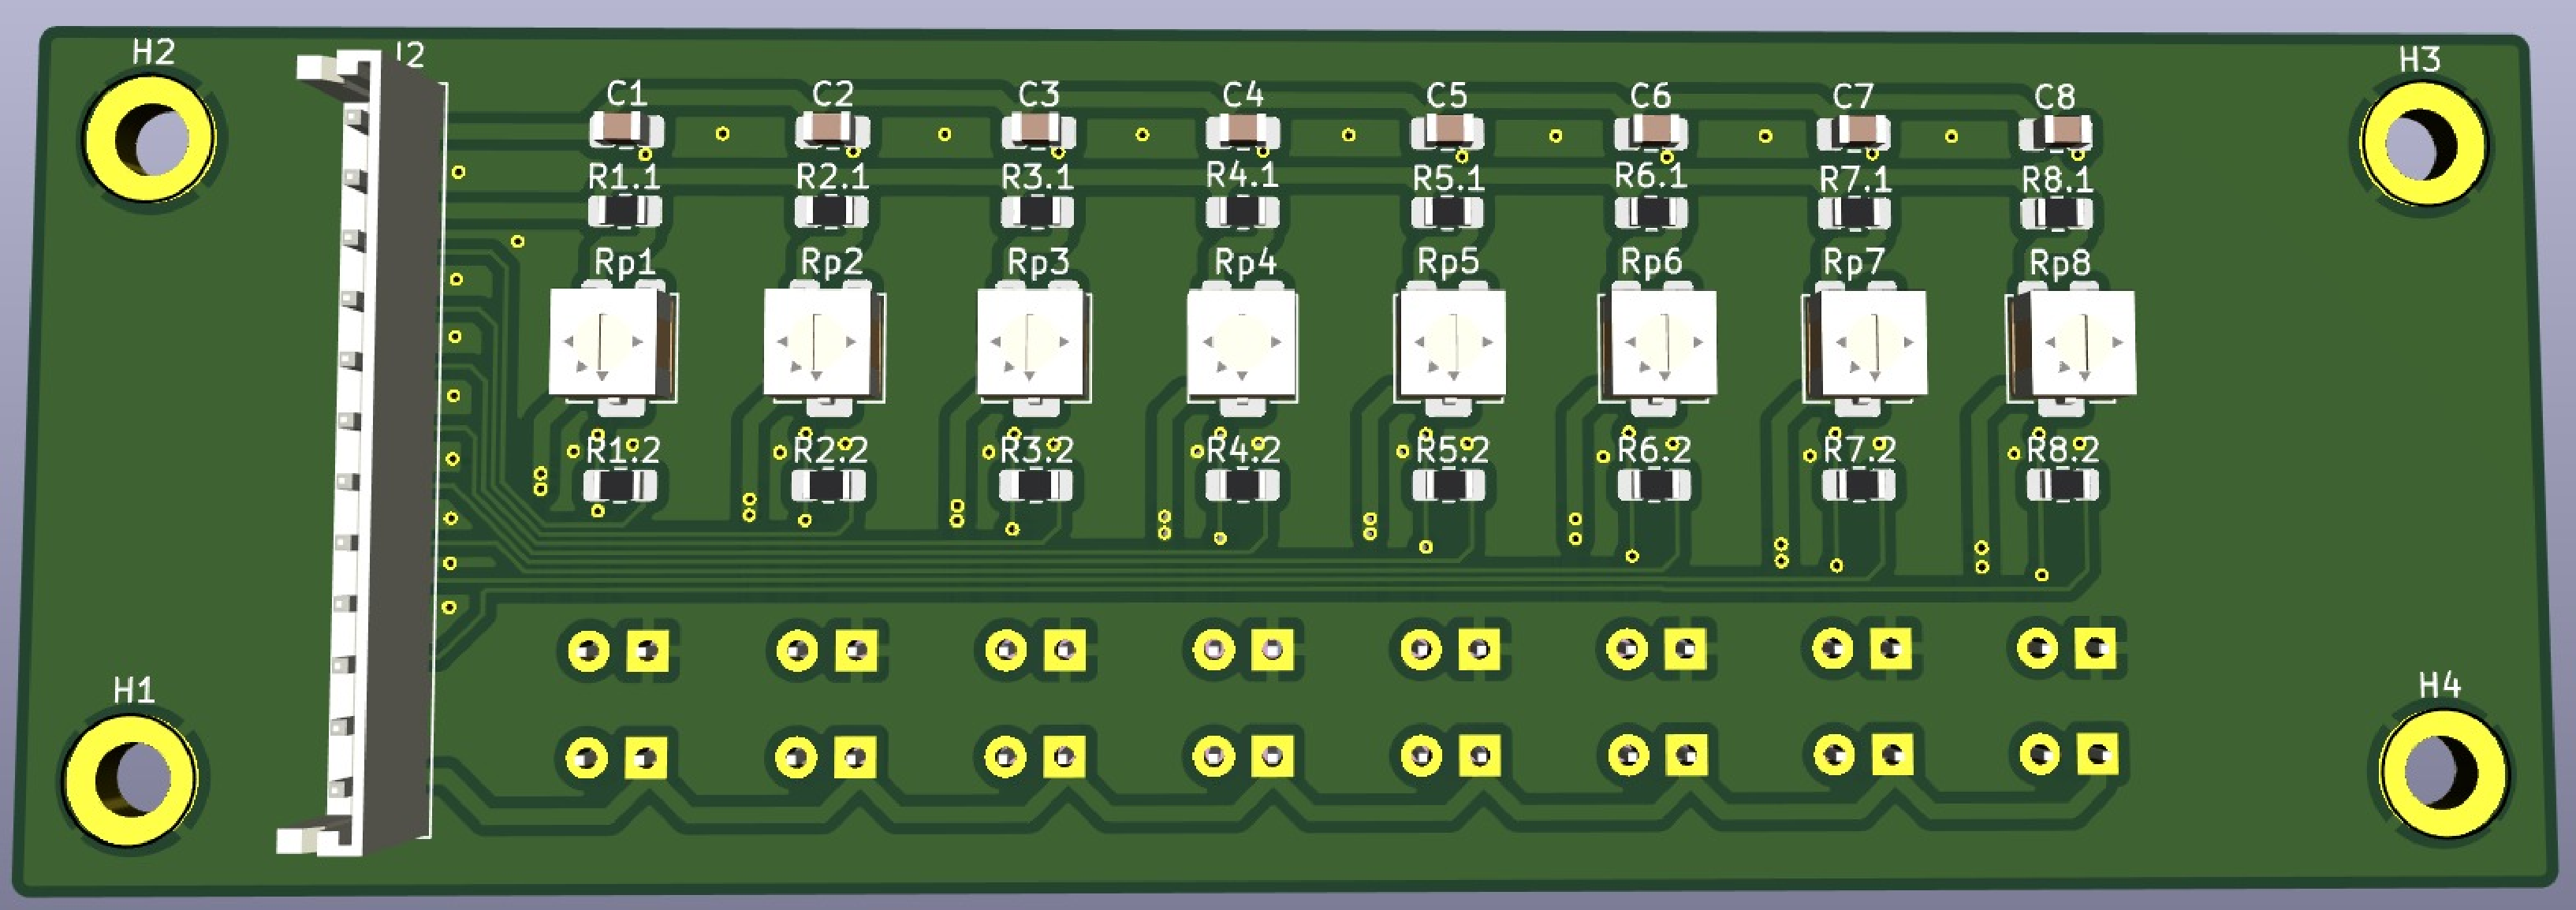
\includegraphics[width=0.75\textwidth]{fig_Strecke_Tracken/Liniensensor_Top.pdf}
    \caption{Liniensensor in Kicad von oben}~\label{fig:Liniensensor_Top}
\end{figure}

\begin{figure}[H]
    \centering
    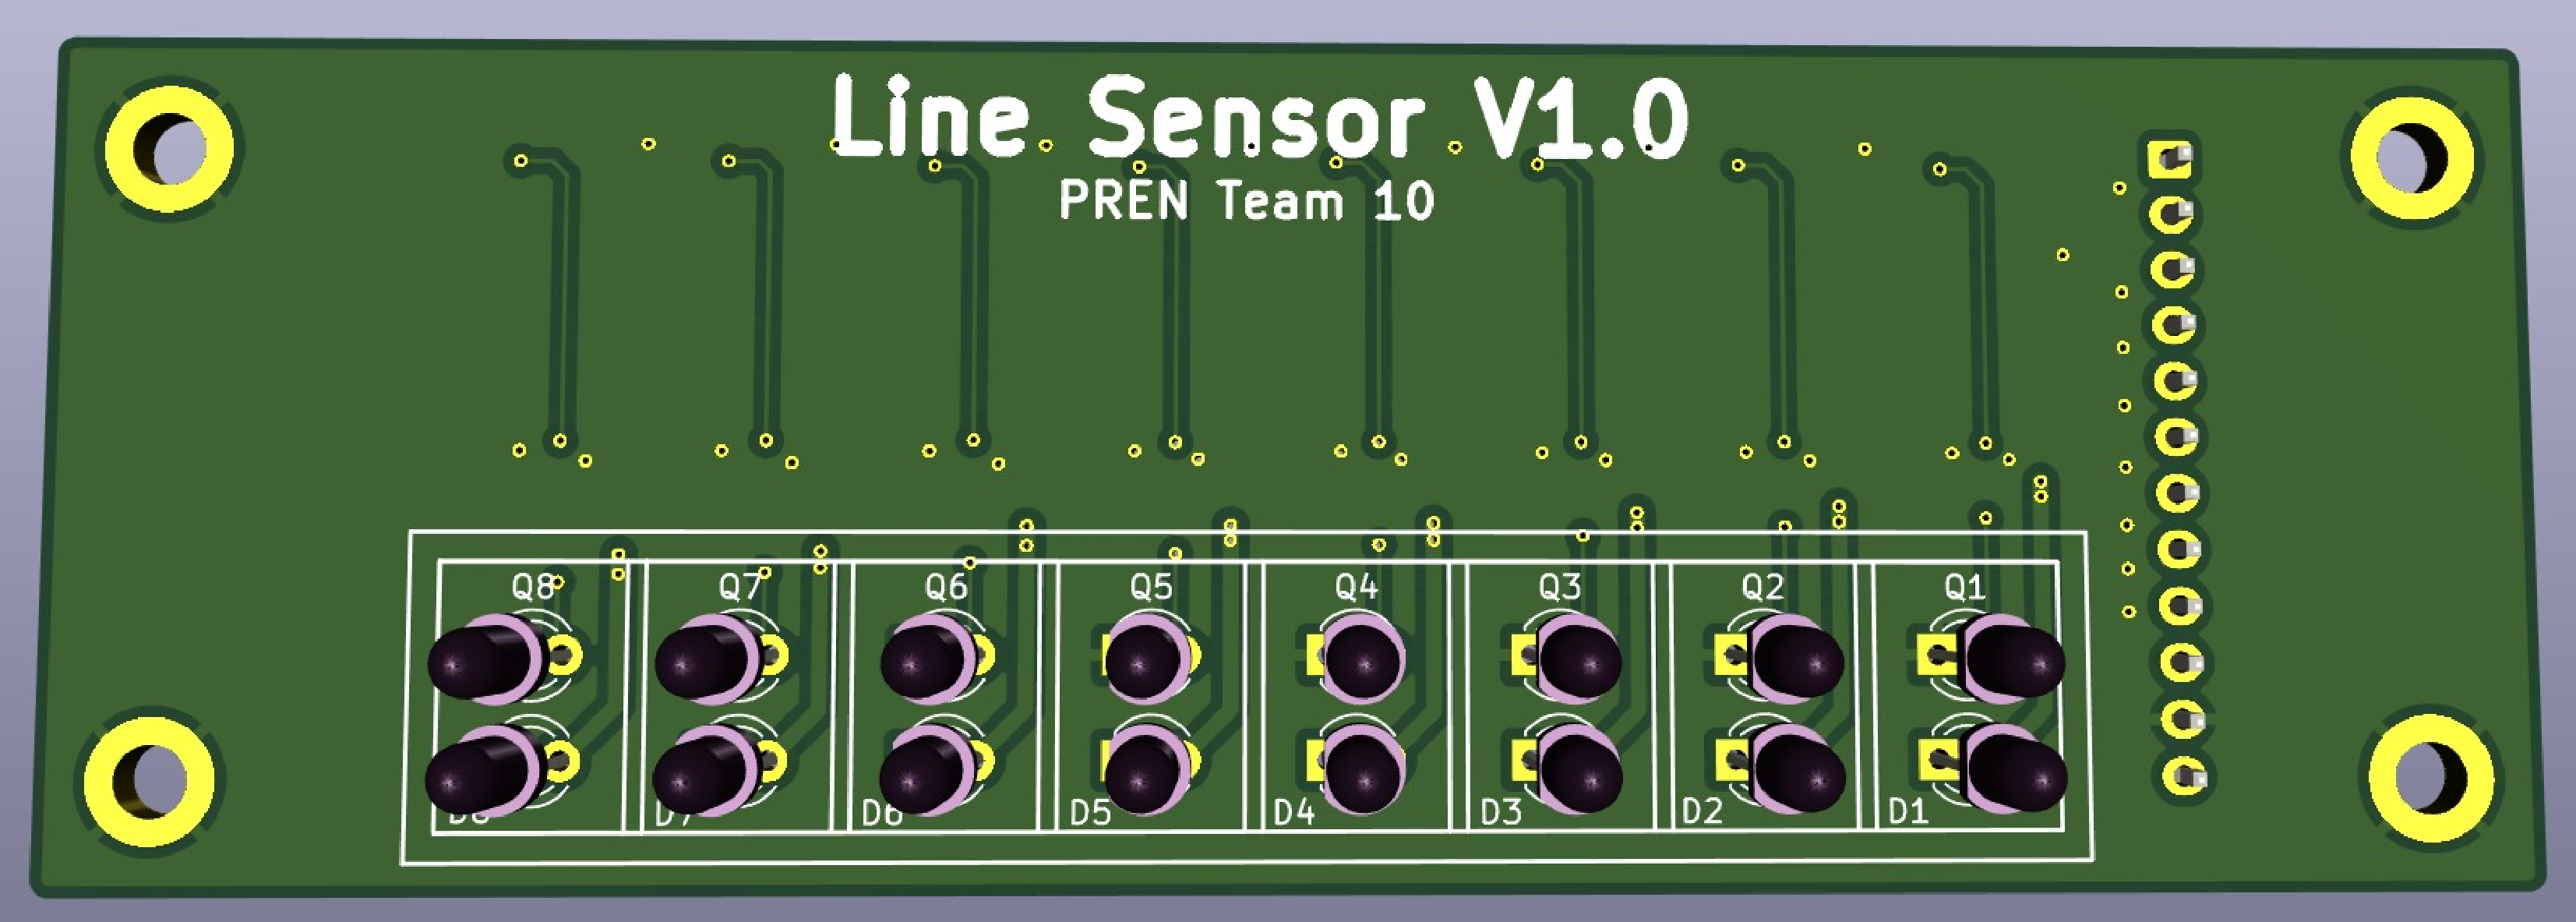
\includegraphics[width=0.75\textwidth]{fig_Strecke_Tracken/Liniensensor_Bottom.pdf}
    \caption{Liniensensor in Kicad von unten}~\label{fig:Liniensensor_Bottom}
\end{figure}

% ===================================================================================

\paragraph{Versuche}
Im Anhang ist ein Versuch dokumentiert, welcher ein geeignetes Lichtspektrum
für den Liniensensor liefert. Ausserdem wurden die Ströme auf den
unterschiedlichen Untergründen (Klebeband, Fliese und Fuge) gemessen. Mittels
eines Arduino sind alle Eingänge ausgewertet und der Liniensensor validiert.
Alle Messungen sind im Anhang~\ref{anhang:Liniensensor} dokumentiert.

% ===================================================================================
\paragraph{Entscheidung und Fazit}
Durch die Messungen wurde das Konzept des Liniensensors überprüft und
validiert. Das folgende Bild bestätigt, dass das Klebeband von der Fliese
deutlich unterschieden werden kann. Die
Abbildung~\ref{fig:Auswertung_Strecke_Beispiel} zeigt die Spannungsauswertung
mittels ADCs. Diese Auswertung wurde mit einem Arduino durchgeführt. Die hohen
Werte stellen die Fliese dar und die tiefen Werte das Klebeband.

\begin{figure}[H]
    \centering
    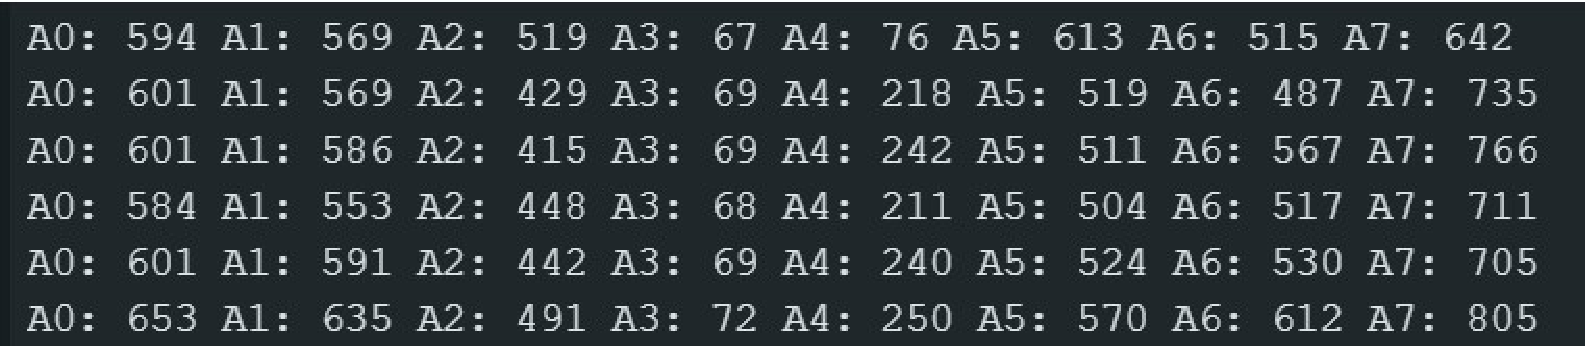
\includegraphics[width=0.75\textwidth]{fig_Strecke_Tracken/Auswertung_Strecke.pdf}
    \caption{Die tiefen Werte stellen das Klebeband dar und die hohen die Fliesen}~\label{fig:Auswertung_Strecke_Beispiel}
\end{figure}

In der Abbildung~\ref{fig:Auswertung_Strecke_Beispiel} ist zu sehen, dass sich
die Zelle A3 direkt über dem Klebeband befindet. Auch die Pins A2 und A4 liegen
teilweise über dem Klebeband. Der Wert ist jedoch grösser, da nur ein Teil des
Klebebandes direkt darunter liegt.

In der Risikobewertung wurde die Unterscheidung zwischen Klebeband und Fugen
als Risiko beurteilt. Der entwickelte Liniensensor ist in der Lage, Fugen von
Klebebändern zu unterscheiden. Dies ist im Anhang~\ref{anhang:Liniensensor}
genauer dokumentiert. Aufgrund der eindeutigen Messwerte wird dieser
Liniensensor verwendet.

\end{document}
